% BACKGROUND & RELATED WORK
%
% !TEX root = ../thesis-main.tex
%
%\chapter{Background and related work}
%\label{chap:background}

%\cleanchapterquote{You can’t do better design with a computer, but you can speed up your work enormously.}{Wim Crouwel}{(Graphic designer and typographer)}

\blindtext 

\chapter{Computer-Assisted Pronunciation Tutoring}
	\blindtext
	\section{Pronunciation in foreign language teaching}
	\section{CAPT systems}
		\subsection{Selecting errors to target}
			\begin{center}
			\begin{figure}[htb]
				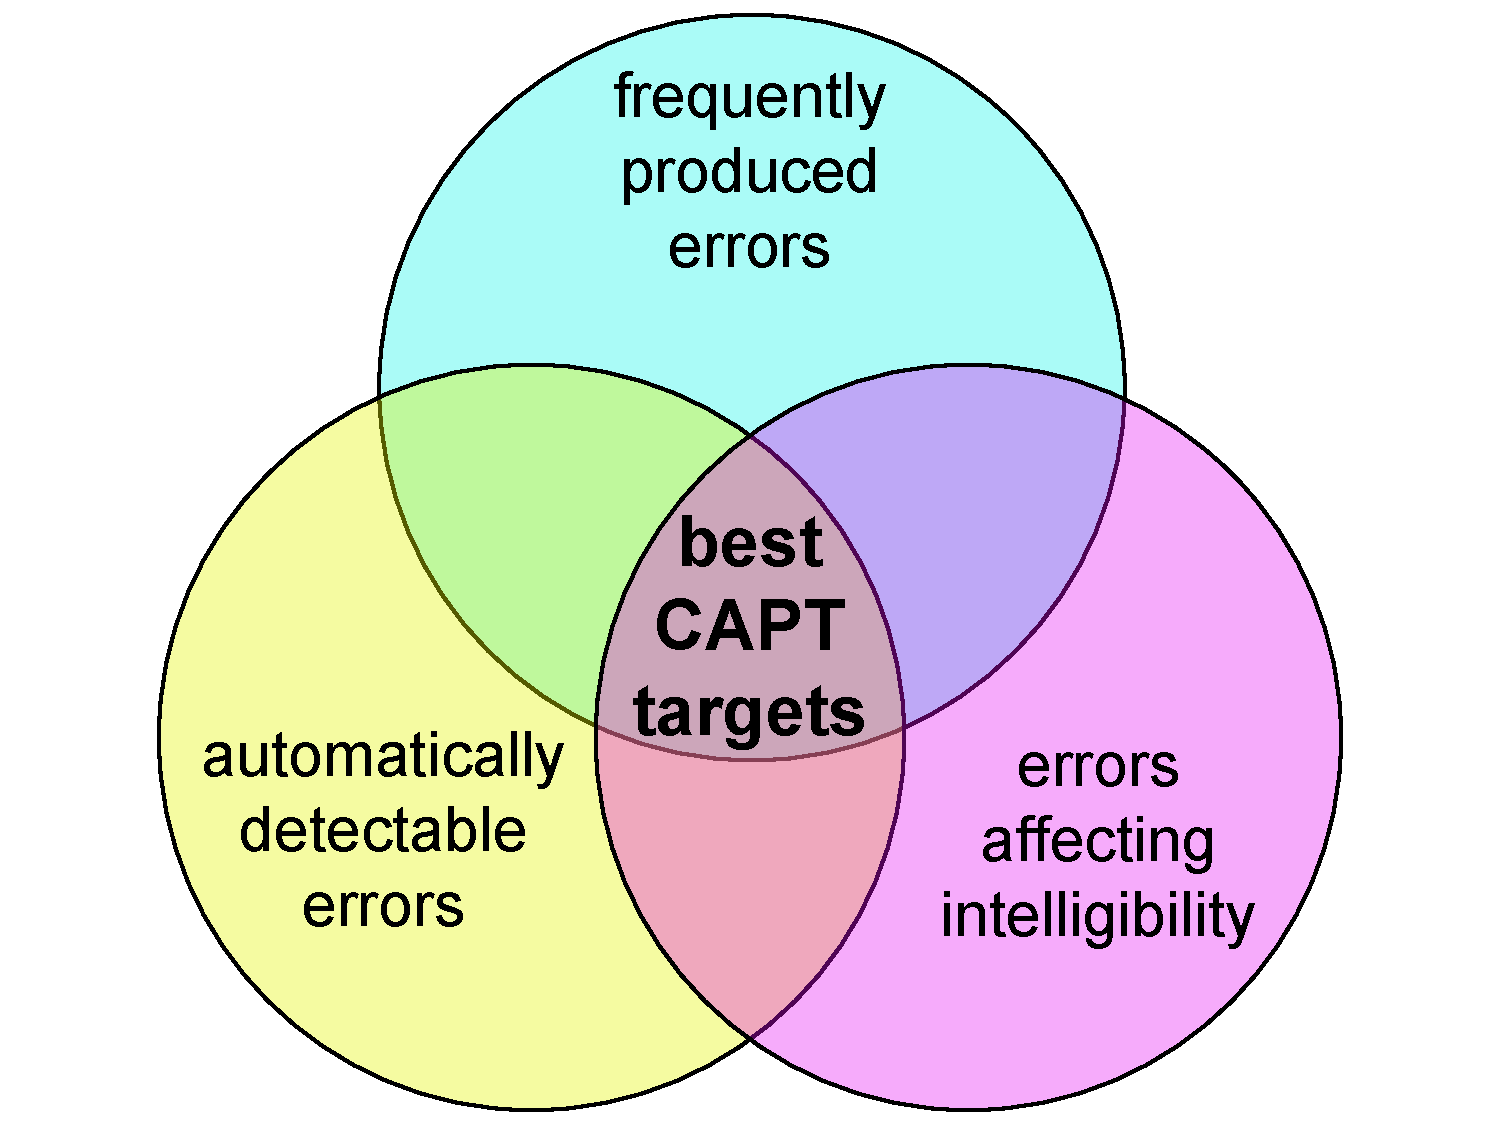
\includegraphics[width=.7\textwidth]{../img/error-venn}
				\caption{Criteria for selecting errors to target in a CAPT system.}
				\label{fig:errors}
			\end{figure}
			\end{center}
		\subsection{Survey of existing CAPT systems}
	\section{The IFCASL project}
		\subsection{Individualized feedback in CAPT?}
		\subsection{The IFCASL corpus}


\chapter{Lexical stress errors for French learners of German}
	\blindtext
	\section{Frequency of production}
		\subsection{Prosody of German vs. French }
		\subsection{Lexical stress errors in the IFCASL corpus} 
	\section{Impact on Intelligibility}
	\section{Automatic detection}